\chapter{Infraestructura}\label{cap.infraestructura}
En este capítulo se explicarán los principales ingredientes software en los que nos hemos apoyado para desarrollar el trabajo. Tales como el simulador Gazebo (con el cual se pueden simular robots con sus sensores y actuadores), el entorno JdeRobot, la biblioteca de OpenCV (empleada en todo lo relacionado con el tratamiento de imagen), PyQt (para el desarrollo de la interfaz gráfica) y Python como lenguaje de programación.

\section{Simulador Gazebo}

Como se argumentó en el Capítulo 1, el simulador Gazebo es uno de los ejes principales de JdeRobot-Academy. Es un simulador usado en robótica que permite realizar diversos escenarios tridimensionales donde probar nuestro software. A la hora de desarrollar el software es necesario hacer pruebas, las cuales saldrían muy costosas si se probaran en robots reales (podría no funcionar correctamente y que el robot se rompiera). Por esta razón es muy útil el empleo de simuladores, pues se pueden realizar las pruebas que se quieran sin peligro de que el robot se estropee. Con los simuladores se pueden diseñar robots y escenarios realistas donde ejecutar los algoritmos creados.

\begin{figure}[H]
  \begin{center}
    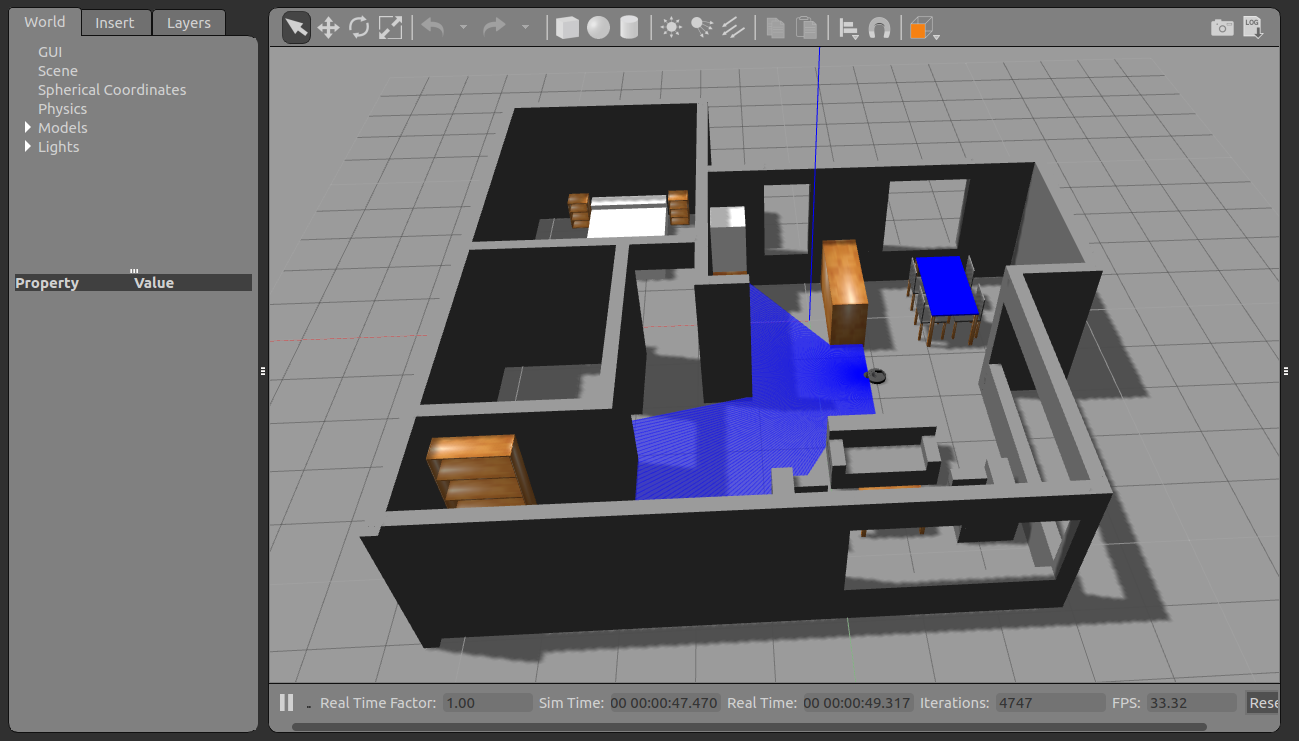
\includegraphics[width=0.8\textwidth]{figures/Infraestructura/gazebo.png}
		\caption{Simulador Gazebo}
		\label{fig.gazebo}
		\end{center}
\end{figure}

 
Gazebo es un programa de código abierto distribuido bajo licencia de Apache 2.0. Se emplea en el desarrollo de aplicaciones robóticas y en inteligencia artificial. Es capaz de simular robots, objetos y sensores en entornos complejos de interior y exterior. Tiene gráficos de gran calidad y un robusto motor de física (masa del robot, rozamiento, inercia, amortiguamiento, etc.). En la Figura~\ref{fig.gazebo} aparece el mundo utilizado en la práctica de ``Aspiradora autónoma con autolocalización''. Se puede apreciar como Gazebo simula tanto objetos (camas, sofás, muebles...) como robots, en este caso, un robot aspirador. \\

Fue elegido para realizar el DARPA Robotics Challenge (2012-2015) y está mantenido por la Fundación Robótica de Código Abierto (OSRF). \\

En este proyecto se emplea la versión 7 de Gazebo, la cual se usará para crear los diferentes entornos y para probar nuestros algoritmos.  Gracias a Gazebo se pueden incluir texturas, luces y sombras en los escenarios, así como simular física como por ejemplo choques, empujes, gravedad, etc. Además, incluye diversos sensores, como pueden ser cámaras y lásers, los cuales podrán ser incorporados en los robots que empleemos. Todo ello hace que sea una herramienta muy potente y de gran ayuda en el mundo de la robótica.\\

Los mundos simulados con Gazebo son 3D, que se cargan a partir de ficheros con extensión ``.world''. Son ficheros definidos en \acrfull{sdf} que es un formato \acrfull{xml} que describe objetos y entornos para simuladores, visualización y control de robots. Originalmente fue desarrollado como parte del simulador Gazebo pero con los años se ha convertido en un formato estable, robusto y extensible capaz de describir todos los aspectos de los robots, los objetos estáticos y dinámicos, la iluminación, el terreno e incluso la física.\\

Se puede describir con precisión todos los aspectos de un robot que usa SDF, ya sea un robot que sea un simple chasis con ruedas o un humanoide. Además de los atributos cinemáticos y dinámicos, se pueden definir sensores, propiedades de superficie, texturas, fricción de la junta y muchas más propiedades para un robot. Estas características permiten usar SDF para simulación, visualización, planificación de movimiento y control de robot. Los modelos de robots que se emplean en la simulación pueden ser creados mediante algún programa de modelado 3D como Blender o Sketchup. Estos robots simulados necesitan ser dotados de inteligencia para lo cual se emplean plugins. Éstos, pueden dotar al robot de inteligencia u ofrecer la información de sus sensores a aplicaciones externas y recibir de éstas comandos para los actuadores de los robots.


\section{Entorno JdeRobot}

\section{Lenguaje de programación Python}

\section{Biblioteca OpenCV}

\section{PyQt}